\section{Durchführung}
\label{sec:Durchführung}
\subsection{Versuchsaufbau}
In diesem Versuch werden die optischen Eigenschaften von Licht untersucht. Dafür werden zwei 
Laser mit unterschiedlicher Wellenlänge als Quelle eines fokussierten Lichtstrahls verwendet.
Der eine Laser emittiert rotes Licht der Wellenlänge $\lambda=\qty{635}{\nano\meter}$ und der andere
grünes Licht der Wellenlänge $\lambda=\qty{532}{\nano\meter}$. In Abbildung \ref{fig:Aufbau1} ist der
generelle Versuchsaufbau dargestellt. Alle Elemente sind auf einer transparenten Grundplatte angeordnet, so
dass verschiedene Vorlagen, wie eine Winkeleinteilung, zur quantitativen Bestimmung der Größen darunter 
platziert werden können. In der Mitte der Platte kann ein zu untersuchendes optisches Element, wie
sie in Abbildung \ref{fig:Aufbau2} dargestellt sind, platziert werden. Der Laser befindet sich
im festen Abstand zur Mitte der Platte. Er kann allerdings in der Winkelposition verändert werden.
Beim Aufbau der optischen Messvorrichtungen ist zu beachten, dass die optischen Elemente nur am 
Rand angefasst werden dürfen, da der Fettfilm die Oberflächen der Elemente beschädigen kann.
\begin{figure}[H]
    \centering
    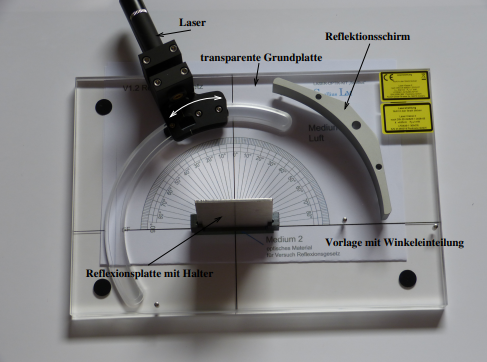
\includegraphics{content/Aufbau1.png}
    \caption{Grundaufbau des Versuchs\cite{V400}}
    \label{fig:Aufbau1}
\end{figure}
\begin{figure}[H]
    \centering
    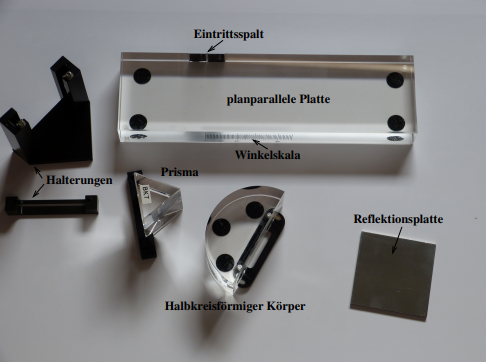
\includegraphics{content/Aufbau2.png}
    \caption{Optische Elemente\cite{V400}}
    \label{fig:Aufbau2}
\end{figure}
\subsection{Untersuchung des Reflexionsgesetz}
Für diesen Versuch wird in der Mitte der Platte eine Reflexionsplatte angebracht.
Als Vorlage wird eine Winkeleinteilung unter die Grundplatte gelegt, sodass Einfalls- und Ausfallswinkel
gemessen werden können. Als Lichtquelle wird der grüne Laser eingeschaltet. Nun wird in jedem Messvorgang
der Einfallswinkel durch Ablesen der Position des Lasers an der Winkelskala gemessen und der Ausfallswinkel wird durch Ablesen
der Winkelposition des auf der Reflexionsplatte auftreffenden Laserstrahls gemessen. Nach jedem Messvorgang wird
die Winkelposition des Lasers verändert, bis 7 Messvorgänge durchgeführt worden sind.
\subsection{Untersuchung des Brechungsgesetz}
Nun wird die Reflexionsplatte durch die planparallele Platte aus Plexiglas ersetzt. Es wird wieder der
grüne Laser verwendet. Das emittierte Licht des Lasers wird nun nicht mehr reflektiert. Stattdessen dringt es in das
Material ein und wird dort gebrochen. Der Einfallswinkel wird wie bei der Reflexion bestimmt. Der Brechungswinkel
lässt sich an einer Skala der planparallelen Platte ablesen. Diese ist so präpariert, dass der Lichtstrahl
an einer bestimmten Stelle eindringt und so dem klar sichtbaren Austrittspunkt einem Brechungswinkel zugeordnet werden kann.
Die Messung wird für 7 verschiedene Einfallswinkel durchgeführt.
\subsection{Bestimmung des Austrittswinkel aus einem Prisma}
In diesem Versuchsteil wird auf die Plattenmitte ein Prisma angebracht. Es werden, wie bei den vorherigen
Versuchen die Einfallswinkel und die Ausfallswinkel zur Flächennormale der Austrittsgrenzfläche gemessen. Für diese Messung
wird eine neue Vorlage, sowie ein spezieller Winkelschirm, verwendet. Der Winkelschirm wird gemäß der Vorlage so
justiert, dass der gut sichtbare Auftrittspunkt des Laserstrahls auf dem Schirm dem Winkel zur Flächennormale entspricht.
Dadurch kann am Schirm dieser Winkel direkt abgelesen werden. Die Messung wird bei 5 verschiedenen 
Einfallswinkeln im Bereich 10° bis 60° und jeweils für beide Laser wiederholt. Da der Laserstrahl im Prisma mehrmals
reflektiert wird, tritt aus verschiedenen Stellen des Prismas ein Strahl heraus. Diese besitzen allerdings eine geringere Intensität
als der zu beobachtende Strahl. Daher wird bei der Untersuchung darauf geachtet nur den austretenden Strahl mit der höchsten
Intensität zu beachten.
\subsection{Bestimmung der Wellenlänge eines Lasers durch Verwendung eines Gitters}
Nun sollen das Interferenzbild eines Gitters untersucht werden. Dafür wird erneut eine neue Winkelskala benutzt.
Diese ist deutlich größer und ermöglicht eine genauere Messung in geringeren Winkelbereichen (0°-30°).
Die Vorlage wird nun allerdings vor die Platte und nicht unter die Platte gelegt. Bevor das Gitter auf die 
eingezeichnete Position gestellt wird, muss der Laser so justiert werden, dass er auch bei genau 0° auf dem, entsprechend der
Vorlage aufgebauten Winkelschirm auftrifft. Daraufhin können die 3 verschiedenen zu Verfügung stehenden Gitter mit
600 Linien/mm, 300 Linien/mm und 100 Linien/mm aufgestellt werden. Die Messung wird bei jedem Gitter und mit beiden Lasern durchgeführt.
Gemessen wird nur der Winkel der einzelnen auf dem Schirm zu beobachtenden Intensitätsmaxima. Jedem Maximum wird
dabei eine Beugungsordnung gemäß der Entfernung zu 0° zugeordnet.
